\documentclass[]{report}
\renewcommand\thesection{\arabic{section}}%for page numbering in arabics
\usepackage{graphicx,tabularx}%for figures and tables
\usepackage[utf8]{inputenc} %allows special characters such as ä, ö, ỳ
\usepackage[english]{babel}  %set the language to English
\usepackage[margin=1.5in]{geometry} %change page margins 
\usepackage{sectsty}%section headers
\allsectionsfont{\sffamily\large}
\subsectionfont{\sffamily\normalsize}
\linespread{1.2}% line distance
\usepackage{lipsum}% http://ctan.org/pkg/lipsum
\usepackage{caption}%use for captions on tables
%use this exact command. The style and bibliographystyle has to be authoryear (Havard). The sorting is nyt: name, year, title so that the bibliography is sorted alphabetically. firstinits=true shortens the names: Albert Einstein -> A. Einstein
\usepackage[backend=bibtex,style=authoryear,bibstyle=authoryear,sorting=nyt,firstinits=true]{biblatex}
\setlength\parindent{0pt}%include this so that your paragraphs don't indent automatically
\addbibresource{report.bib} %this attaches your bib-file, your bibliography (must be in the same folder)
\usepackage[compact]{titlesec}%include title formatting package
\graphicspath{ {./images/} }

% Title Page
\title{Git CLI or GitHub Desktop \\ What are the factors that influence the choice of the interface among IT students?}
\author{Danil Burov and Giulio Raffaeli}
\date{December 18th 2023\\Module: ARDA \\Venlo, Limburg, Netherlands}


\begin{document}
	
	\maketitle
	
	\begin{abstract}
		%history%
		When it comes to learning programming one of the main aspects an IT student needs to learn is how to version control (VS) their work. The most common tool for versioning is Git. In the beginning IT students need to choose between Command Line Interface (CLI) and Graphical User Interface (GUI) for Git usage. \\\\
		%cite -> wikipedia% 
		%topic introdutction%
		
		This purpose of this research is to identify what are the main factors that influences the choice of the interface among IT students. In order to evaluate the reasons, a survey was conducted. Since the most efficient way of using Git is through the CLI an experiment was done to understand why students adhere to the GUI instead switching to the more efficient interface.\\\\
		%data evaluation%
		The results show that the majority of IT students prefer using Git through the GUI, finding it more visual appealing and easier to understand. Even thought, students that CLI is more efficient using Git they still use the GUI because making the transition is harder than sticking to the interface. This statement is proven with our experiment.\\\\
		\pagenumbering{roman}
		
	\end{abstract}
	\tableofcontents
	\setcounter{page}{3}
	\listoffigures %UNCOMMENT IF YOU HAVE FIGURES
	%\listoftables %UNCOMMENT IF YOU HAVE TABLES
	\pagebreak
	
	\pagenumbering{arabic}	
	
	\section{Introduction}
	The purpose of this chapter is to provide the research question and the importance of it, along with context about the topic. Furthermore, this chapter will point out potential external factors that may influence the evaluation of the hypothesis and its sub-questions. \\
	\subsection{Context and Background}
	
	%Talk about how Git works%
	\subsubsection{Git}
	Up until this date Git is the most popular versioning control system, used by more than 93 percent of developers ('cite' -> StackOverflow survey). In order to understand Git it is crucial to know what is a versioning control system is (VCS). It is a system that enables developers to keep historical version of source code(*) and project files that are under development and retrieve past version. It is required when developing projects above a few hundred lines of code or where more than one developer needs to collaborate on a project. It stores version information for every file in what is generically called - 'repository'('cite -> pdf history of version control') . The basic structure of a Git repository has three main components. First, a .git directory which has the functionality of storing the meta data and object database for you repository and all the committed changes. Second, a staging area where new features that still need to be committed are kept, waiting for a commit to take place. Lastly, a working directory where your plain running copy of the source code is held. Once a commit takes place, the changes are saved from the staging area to the .git directory. ('cite -> pdf for CLI compare to GUI').
	
	\subsection{Command line Interface and Graphical User Interface}
	%Story CLI vs GUI%
	When the first personal computer was invented in 1973 (Kenbak - 1) ('cite' - > Museum computerhistory.org) users were forced to use the command line interface as their only way of interacting with the machine. Later on, with more people using the personal computers the need for a graphical user interface increased. The first prototypes of personal computers that use the GUI were developed in the 1970s (XEROX Alto 1973) ('cite' -> wikipedia), however, it became popular with the release of the 'Macintosh' in 1984. ('cite' ->wikipedia ). From that point on, the majority of users started using the GUI as their main interface relegating the use of CLI only to a small percentage of users.\\
	When Git was first released in 2005 ('cite' -> Gitpage) the only way to work with it was through the command line interface. Throughout the years many graphical user interfaces supporting Git were developed with the most important one being GitHub Desktop, created in 2017. ('cite' -> GitHub page)
	
	%How they work with Git%
	%Which one is more efficient%
	%two of the main limiting factors when it comes to the GUI
	When using the command line interface you type commands manually to perform the desired actions whilst in a graphical user interface you will have something visual to interact with, such as buttons, input fields and so on. There are advantages and disadvantages of using either of the two interfaces not only for Git but in general. ('cite' -> pdf for CLI vs GUI). When it comes to programming, 83('cite' -> StackOverflow survey) percent of developers prefer the CLI instead of the GUI for various of reasons. Here are some of them: \\1) Interaction speed, when it comes to GUI the speed is determined mostly on how fast you can navigate with your mouse and click speed while with the CLI what you need to do is just interact with the keypad making the process faster. \\2) Efficiency, because of the way interaction is handled in the GUI it also requires more actions compared to the CLI to execute the same task. For example: If you want to commit changes to the main repository with the CLI you need to execute three consecutive commands, whereas in the GUI you need to navigate through three different buttons and you have to input a message with your keyboard. \\3) One complaint about CLI tools is that they supposedly have a 'steeper learning curve' and no one can remember what commands to use. However, if you need to learn a complex GUI the 'learning curve' can be as steep as learning the CLI. Although, in the long run it is always better to the learn the CLI because more efficient. ('cite' -> github repo)

	%Reasearch question% 
	%hypothesis -> X -> Y potential C's and I's%
	\section{Research questions and Hypothesis}
	The aim of the research is to find what are the reasons that influence the choice of the interface among IT students. Therefore our research questions is: "What are the factors that influence the choice of the interface among IT students?". Since surveys show that command line interface is more used ('cite' -> StackOverflow ) than graphical user interface ('cite' -> GitHub repo) and also more efficient the sub-question this research paper is aiming to answer is the following: "Is transitioning to the CLI hard for an IT student that still uses the GUI?".
	
	We hypothesis that students do not base their choice of Git interface on efficiency but on how user-friendly and simple the interface is. Therefore, we also believe that making the transition to the CLI from GUI is hard, because of the steep learning curve from the beginning and that is why IT students keep using the GUI.\\
	Although, there are some external factors that need to be taken into consideration. \\1) The years a student has already programmed for.\\2) How long have they been working with Git. \\3) What was their first chosen interface.\\4) Which operating system do they use. \\
	
	In order to take into consideration the given factors a survey was conducted to evaluate what are the aspects that influence the choice of interface for an IT student. Parallel to the survey, an experiment was conducted with students that have never used the CLI before in order to understand what difficulties they will encounter when learning basic commands and if it makes them faster at using Git. 
	
	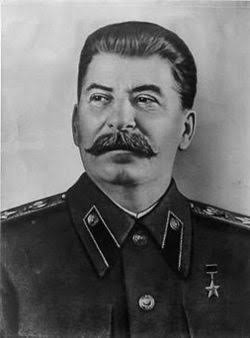
\includegraphics{test}
	
	\chapter{Methodology}
	This chapter will explain how we performed our research and how we set up our comparative analysis.
	
	\section{Gathering data}
	\subsection{Survey}
	
	In order to answer our main question, while also keeping in consideration all the external variables that may influence the answer, a survey was conducted.
	Since the research aims to give an answer that represents all IT students, the survey was sent not only to Fontys learners, but also to students from other universities.
	The survey itself consists of 14 multiple choice questions, plus an optional open question. It is structured as follows:\\
	First of all general questions are asked, regarding how long has the participant programmed for, how long has he been using Git and what is his current knowledge of the tool.
	Next questions are related to which Operating System does the responder primarily use and how did he get into Git at first (from which sources did he learn to use it and with which interface).
	Afterwards, information regarding which interface does the participant currently use and why is gathered
	Subsequently, the respondent needs to associate various words to both interfaces, in order to understand what is his opinion on them.
	Lastly, questions about whether the candidate has ever considered switching interface and if he thinks that doing so would improve his efficiency are asked.
	In order to easily convert all the answers into data, the survey was created with the tool Google Forms (Google - 2008).
	The list of all the questions and the possible replies can be found in the appendix.
	
	\subsection{Experiment}
	
	%i have stated that experienced users have conducted the experiment as well and results show that since they have prior knowledge with the CLI it was easier for them to complete the exercise without any problem%
	
	%i will specify that we have made an experiment with 5 people that have never used Git with CLI and 5 people who have already used Git with CLI%
	
	%the purpose of the assignment%
	The main purpose for the experiment conducted for our research paper is to prove that when a person wants to switch from using the graphical user interface (GitHub Desktop) for Git to the command line interface the transition will take time and effort when it comes down to getting used to the commands. Especially because as mentioned above the learning curve is very steep. ('cite' -> GitHub repo).
	%questionable :D%
	
	%explaining why we are doing two experiments with gui and cli and why we are doing the assignment briefly%
	The exercise given to the students represent a very simple scenario where a developer would need to use Git through their interface. For the sake of our paper the experiment was done through both the graphical user interface and the command line. For a GUI we chose to use 'GitHub Desktop' since it is the most commonly used graphical interface ('cite' -> find somewhere to cite from this quote). The purpose of doing the assignment in both the interfaces is to prove that using the CLI for Git is much slower for students who have never used it and much more confusing. However, when a student had already used the CLI for Git purposes it was seen that the issues the newcomers had (mainly commands) weren't in the picture.\\
	
	%explaining the assignment%
	The assignment is covering all the basic commands that need to be done in order to complete a commit changes in a repository. Both groups of IT students have never seen the assignment and were treated as they have never used Git through the CLI. They were given two sheets of paper and a repository containing the assignment they need to complete. The first paper, contained all the commands required to complete the assignment ('refer to a figure').The second paper, had the description of the assignment.('refer to a figure here'). Time was recorder during the conducting of the exercises.
	
	
	\section{Data visualization and transformation}
	 Whereas, using 'GitHub Desktop' for the assignment showed a significantly better result when it comes down to speed and understandment 
	%Research model -> research methods%
	%Survery%
	%Experiment%
	\chapter{Results}
	%Survery results%
	%Experiment results%
	%Data analysis%
	\newpage	
	\chapter{Discussion}
	%Result interpration%
	%Evaluate research questions%
	%Limitations -> Y factors%
	%further research%
\end{document}


\printbibliography[title=References]

\end{document}          
